The general equation of a second degree can
be expressed as:
\begin{align}
a{x^2}+2b{xy}+c{y^2}+2d{x}+2e{y}+f=0\label{eq:solutions/41/20/geneqn}\\
   \Longrightarrow \vec{x^TVx}+2\vec{u^Tx}+f=0\label{eq:solutions/41/20/geneqn2}
\end{align}
where\begin{align}
\vec{V} =\myvec{a\quad b\\b\quad c},\vec{u}=\myvec{d\\e}\label{eq:solutions/41/20/paraeqn} 
\end{align}
The given equation of the curve can be expressed as:
\begin{align}
    40{x^2}+2(18){xy}+25{y^2}+2(-98){x}+2(-61){y}+205=0\label{eq:solutions/41/20/giveneqn}
\end{align}
Comparing \eqref{eq:solutions/41/20/geneqn},\eqref{eq:solutions/41/20/paraeqn} and \eqref{eq:solutions/41/20/giveneqn}:\\
\begin{align}
\vec{V} = \myvec{40\quad\sqrt{18}\\\sqrt{18}\quad 25},\vec{u}=\myvec{-98\\-61} and\quad f=205 \\
       \Longrightarrow\mydet{\vec{V}}=982\quad and \quad b^2-ac=18-40.25 =-982
\end{align}
Since $\mydet{\vec{V}}>0$\quad and \quad $b^2<ac$ , \eqref{eq:solutions/41/20/giveneqn} represent an ellipse. \\
 The characteristic equation of $\vec{V}$ is given as follows,
\begin{align}
\mydet{\lambda\vec{I}-\vec{V}} = \mydet{\lambda-40\quad\sqrt{18}\\\sqrt{18}\quad\lambda -25} &= 0\\
\implies \lambda^2-65\lambda+982 &= 0\label{eq:solutions/41/20/eqchar}
\end{align}
Hence the characteristic equation of $\vec{V}$ is given by \eqref{eq:solutions/41/20/eqchar}. The roots of \eqref{eq:solutions/41/20/eqchar} i.e the eigenvalues are given by
\begin{align}
\lambda_1=\frac{65+\sqrt{297}}{2}, \lambda_2=\frac{65-\sqrt{297}}{2}\label{eq:solutions/41/20/eqeigenvals}    
\end{align}
The eigen vector $\vec{p}$ is defined as, 
\begin{align}
\vec{V}\vec{p} &= \lambda\vec{p}\\
\implies\brak{\lambda\vec{I}-\vec{V}}\vec{p}&=0\label{eq:solutions/41/20/eqneigvenvec}
\end{align}
for $\lambda_1=\frac{65+\sqrt{297}}{2}$,
\begin{align}
\brak{\lambda_1\vec{I}-\vec{V}}=\myvec{\frac{\sqrt{297}-15}{2}&-\sqrt{18}\\-\sqrt{18}&\frac{\sqrt{297}+15}{2}}\\\xleftrightarrow{R_2=R_2+\frac{2\sqrt{18}}{\sqrt{297}-15}R_1}\myvec{\frac{\sqrt{297}-15}{2}&-\sqrt{18}\\0&0}\label{eq:solutions/41/20/norm eqn1}
\end{align}
From \eqref{eq:solutions/41/20/eqneigvenvec} and \eqref{eq:solutions/41/20/norm eqn1}
\begin{align}
\implies\vec{p_1}&=\myvec{\sqrt{18}\\\frac{\sqrt{297}-15}{2}}
\end{align}
For $\lambda_2=\frac{65-\sqrt{297}}{2}$
\begin{align}
\brak{\lambda_2\vec{I}-\vec{V}}=\myvec{\frac{-\sqrt{297}-15}{2}&-\sqrt{18}\\-\sqrt{18}&\frac{15-\sqrt{297}}{2}}\\
\xleftrightarrow[R_1=-R_1]{R_2=R_2+\frac{2\sqrt{18}}{\sqrt{297}+15}R_1}\myvec{\frac{\sqrt{297}+15}{2}&\sqrt{18}\\0&0}
%\label{eq:solutions/41/20/norm eqn1}
\\
\implies\vec{p_2}=\myvec{-\sqrt{18}\\\frac{\sqrt{297}+15}{2}}
\end{align}
 \quad using the affine transformation
\begin{align}
\vec{x}&=\vec{P}\vec{y}+c
^{\prime}\intertext{such that}
\vec{P}^T\vec{V}\vec{P}=\vec{D}\quad and\quad\vec{P}&=\myvec{\vec{p_1}&\vec{p_2}},\quad\vec{P}^T=\vec{P}^{-1}\\
\intertext{Where $\vec{D}$ is a diagonal matrix, we get}
\vec{D}&=\myvec{\frac{65+\sqrt{297}}{2}&0\\0&\frac{65-\sqrt{297}}{2}}
\end{align}
Now \eqref{eq:solutions/41/20/geneqn2} can be written as,
\begin{align}
\vec{y^T}\vec{D}\vec{y}&=\vec{u^T}\vec{V^{-1}}\vec{u}-f\quad\text{$\mydet{\vec{V}}\not=0$}\label{eq:solutions/41/20/eqnewmain}\\
\intertext{And,}
\vec{c^\prime}&= -\vec{V^{-1}}\vec{u}\qquad\text{$\mydet{\vec{V}}\not=0$}\label{eq:solutions/41/20/eqcenter}\\
\vec{y} &= \vec{P^T}\brak{\vec{x-c}}\label{eq:solutions/41/20/eqY}
\end{align}
The centre of the conic section in \eqref{eq:solutions/41/20/giveneqn} is given by $\vec{c^\prime}$ in \eqref{eq:solutions/41/20/eqcenter}. 
We compute $\vec{V^{-1}}$ as follows,
\begin{align}
\myvec{40&\sqrt{18}&1&0\\\sqrt{18}&25&0&1}&\xleftrightarrow[R_1=\frac{1}{40}R_1]{R_2=R_2-\frac{\sqrt{18}}{40}R_1}\myvec{1&\frac{\sqrt{18}}{40}&\frac{1}{40}&0\\0&\frac{982}{40}&-\frac{\sqrt{18}}{40}&1}\\
&\xleftrightarrow[R_1=R_1-\frac{\sqrt{18}}{40}R_2]{R_2=\frac{40}{982}R_2}\myvec{1&0&\frac{25}{982}&-\frac{\sqrt{18}}{982}\\0&1&-\frac{\sqrt{18}}{982}&\frac{40}{982}}
\end{align}
Hence $\vec{V^{-1}}$ is given by,
\begin{align}
\vec{V^{-1}} = \myvec{\frac{25}{982}&-\frac{\sqrt{18}}{982}\\-\frac{\sqrt{18}}{982}&\frac{40}{982}}
\end{align}
Now $\vec{u^T}\vec{V^{-1}}\vec{u}$ is given by,
\begin{align}
\vec{u^T}\vec{V^{-1}}\vec{u}&=\frac{1}{982}\myvec{-98&-61}\myvec{25&-\sqrt{18}\\-\sqrt{18}&40}\myvec{-98\\-61}\\&=344.4203\label{eq:solutions/41/20/eqRHS}\\
\intertext{And, $\vec{V^{-1}}\vec{u}$ is given by,}
\vec{V^{-1}}\vec{u} &= \frac{1}{982}\myvec{25&-\sqrt{18}\\-\sqrt{18}&40}\myvec{-98\\-61}\label{eq:solutions/41/20/eqcenterRHS}\\
\end{align}
By putting the value of \eqref{eq:solutions/41/20/eqcenterRHS}, the center of the ellipse is given by \eqref{eq:solutions/41/20/eqcenter} as follows,
\begin{align}
\vec{c^\prime} = \myvec{2.231\\2.061}
\end{align}
Also the semi-major axis ($a$) and semi-minor axis ($b$) of the ellipse are given by,
\begin{align}
a = \sqrt{\frac{\vec{u^T}\vec{V^{-1}}\vec{u}-f}{\lambda_1}}=1.8414\\
b = \sqrt{\frac{\vec{u^T}\vec{V^{-1}}\vec{u}-f}{\lambda_2}}=2.416
\end{align}
Finally from \eqref{eq:solutions/41/20/eqnewmain}, the equation of ellipse is given by,
\begin{align}
&\vec{y^T}\myvec{41.116&0\\0&23.883}\vec{y}=139.4203\label{eq:solutions/41/20/eqFinal}
\end{align}
\begin{figure}[!]
 \begin{center}
  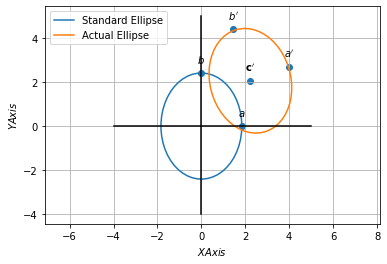
\includegraphics[width=\columnwidth]{solutions/41/20/assignment6_fig.png}
    \caption{Graphical representation of the actual curve  $40{x^2}+36{xy}+25{y^2}-196{x}-122{y}+205=0$, which represent an ellipse.}
\label{eq:solutions/41/20/myfig:1}
    \end{center}
\end{figure}
